% !TEX root = main.tex

\section{Graph-based inertial-kinematic odometry}

We describe the inertial-kinematic odometry for legged robots, based on a graph model. 

%%%%%%%%%%%%%%%%%%%%%%%%%%%%%%%%%%%%%%%%%%%%%%%%%%%%%%%%
\subsection{Graph-based iterative optimization}

In graph-based optimization, the problem is represented as a graph, where the nodes refer to the variables and the factors (or edges) represent the geometrical constraints between variables, produced by the measurements.
%
The state $\bfx$ is modeled as a multi-variate Gaussian distribution, and includes, in our case (see \figRef{fig:factor_graph}), foot poses and velocities $(\bfp,\bfq,\bfv)$ and IMU biases $(\bfa_b,\bw_b)$ at selected keyframes (KF) along the trajectory.
%
For each factor, we can define an error or residual $\bfr$ as the discrepancy between a measurement $\bfz$ and its expectation given the involved state variables,
%
\begin{equation}
    \bfr(\bfx) = h(\bfx) + \bfv - \bfz, \qquad \bfv \sim \mathcal \cN (0, \bfOmega\inv)\label{eq:error}
\end{equation}
%
being $h(\bfx)$ the sensor measurement model and $\bfOmega$ the information matrix of the measurement Gaussian noise $\bfv$.
Importantly, the functions $h(\bfx)$ and $\bfr(\bfx)$ are very sparse, since only a small handful of blocks of $\bfx$ are involved in each factor, which results in a loosely connected graph.
In case of variables defined in manifolds, such as quaternions or rotation matrices, (\ref{eq:error}) becomes $\bfr(\bfx) = (h(\bfx) \oplus \bfv) \ominus \bfz$, with $\bfJ_k = \partial (h_k(\bfx)\ominus\bfz_k)/\partial \Delta \bfx$. 
The $\oplus$ and $\ominus$ are the addition and subtraction operators on the manifold, as required for certain state blocks intervening in the factor (see \eg~\cite{Smith_arv90}, \eqRef{equ:imu_residual} in \secRef{sec:imu}, or \eqsRef{equ:plus_q}{equ:minus_R} in \appRef{sec:derivatives_SO3}).

The maximum a posteriori estimation is obtained by iteratively minimizing the Mahalanobis squared norm of all linearized errors
%
\begin{align}
  \Delta \bfx^* &= \argmin_{\Delta \bfx} \sum_k \norm{ \bfr_k(\breve\bfx) + \bfJ_k \Delta \bfx }_{\bfOmega_k^{-1}}^2 \label{eq:LeastSquares}
\end{align}
%
being $\breve\bfx$ the state estimate at the current iteration, and $\bfJ_k$ the Jacobian of the $k$-th residual $\bfr_k(\bfx)$.
%
Current methods use Cholesky \cite{Kummerle_icra11,ila_ijrr17} or QR  \cite{Dellaert_ijrr06,Kaess_ijrr11} matrix factorizations to solve for $\Delta\bfx^*$, which is used to update state. 
The process is iterated until convergence.
%
Incremental methods \cite{Kaess_ijrr11,ila_ijrr17}, update the problem directly on the factorized matrix, obtaining important speed-ups.


%%%%%%%%%%%%%%%%%%%%%%%%%%%%%%%%%%%%%%%%%%%%%%%%%%%%%%%%%

%Estimation is realized with a tool in ongoing development \textbf{(cite WOLF ?)} and using Google Ceres non-linear least squares optimizer. This optimization is run on data given by the front-end part of the framework,
%which aim is to formalize the problem according to the graph-based model for aforementioned reasons. This representation, illustrated in \figRef{fig:factor_graph}, 
%gives a human-readable way to easily visualize optimized states (circles) linked to constraining information during the optimization process (factors drawn as squares). Constraints are set by the front-end process using measurements from sensors.
%Thus, it is possible to constrain states with several factors provided by different sensors leading to a fusion. Factor play a key role since they are used on top of previous states to predict next ones and compute the error with the current states.
%The optimal states are computed so that the overall residual is minimized in a least squares meaning.

%\subsection{The inertial-kinematic odometry}
%\subsubsection{Inertial pre-integration}
%\subsubsection{Graphical model}

\begin{figure}[tb]
\centering
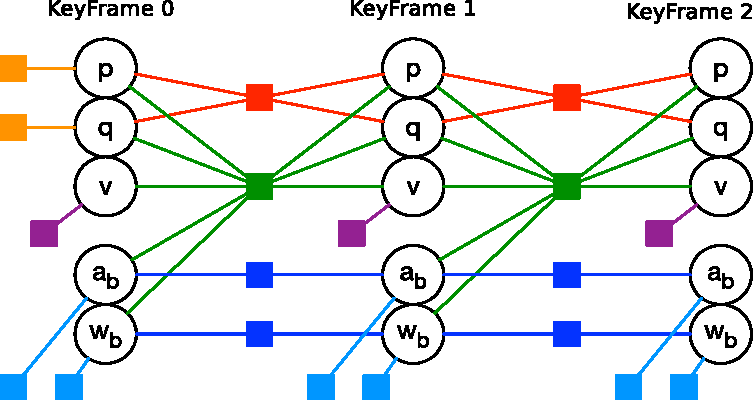
\includegraphics[scale=0.65]{figures/graph_exploded}
\caption{
{\bf Top}: Detailed factor graph for the initial keyframe and two steps. 
\emph{Circles}: state blocks for position ($\bfp$), orientation quaternion ($\bfq$), velocity ($\bfv$), accelerometer bias ($\bfa_b$), gyrometer bias ($\bw_b$). 
\emph{Orange}: initial pose factor. 
\emph{Red}: leg kinematic factor. 
\emph{Purple}: zero-velocity factor. 
\emph{Green}: IMU's delta pre-integration factor. 
\emph{Blue}: bias drift factor. 
\emph{Cyan}: bias absolute factor. 
%{\bf Bottom}: Equivalent factor graph exhibiting one aggregate state block $\bfx=(\bfp,\bfq,\bfv,\bfa_b,\bw_b)$ for each key-frame. All factors are affecting exactly the same variables as in the Top graph.
}
\label{fig:factor_graph}
\end{figure}



%%%%%%%%%%%%%%%%%%%%%%%%%%%%%%%%%%%%%%%%%%%%%%%%%%%%%
%\subsection{Graph-based inertial-kinetic odometry}

\subsection{Keyframe variables}

During a biped walk, we take profit of certain situations where precise assumptions can be made. For example, the  foot velocity is null during the support phase. At these selected moments, we create the keyframes that will produce a chain of states. These are linked by the measurements, forming our factor graph. The KF state blocks are the foot's position, velocity and orientation quaternion, plus the IMU's accelerometer and gyrometer biases,
%
\begin{align}
\bfx_i = \begin{bmatrix}
\bfp_i & \bfv_i & \bfq_i & \bfa_{b,i} & \bw_{b,i}
\end{bmatrix}\tr
~.
\end{align}
%


%%%%%%%%%%%%%%%%%%%%%%%%%%%%%%%%%%%%%%%%%%%%%%%%%%%%%
\subsection{Description of factors}

The types of factor considered in our graph are illustrated in \figRef{fig:factor_graph}. 
Each factor requires its own information matrix $\bfOmega_k$, which is individually specified.

\subsubsection{Absolute factors}

These include initial position and orientation (yellow in the figure), zero velocity (purple), and bias magnitude (cyan). They all define a residual which depends on a single state block, which is compared against a reference $\bfz_k$,
%
\begin{align}
\bfr_k(\bfx) = \bfphi_i - \bfz_k
\end{align}
%
where $\bfphi_i$ is one amongst $\{\bfp_i,\bfv_i,\bfa_{b,i},\bw_{b,i}\}$. 
For the quaternion we implement a residual in the $S3$ manifold,
%
\begin{align}
\bfr_k(\bfx) = \Log(\bfz_k^*\ot\bfq_i)
\end{align}
%

\subsubsection{Bias drift factors}

These are relative factors that allow the biases to drift with time at a controlled rate. Their residual depends on two state blocks, namely
%
\begin{align}
\begin{split}
\bfr(\bfa_{b,i}, \bfa_{b,j}) &= \bfa_{b,j} - \bfa_{b,i} 
\\
\bfr(\bw_{b,i} , \bw_{b,j})  &= \bw_{b,j}  - \bw_{b,i}
\end{split}
\end{align}

\subsubsection{Kinematic chain factors}

These relate position and orientation of consecutive steps, corresponding to the robot's kinematic chain as measured by its joint encoders,
%
\begin{align}
\bfr(\bfp_i,\bfq_i,\bfp_j,\bfq_j) = \begin{bmatrix}
\bfp_j-\bfp_i \\
\Log(\bfq_i^*\ot\bfq_j)
\end{bmatrix}
\end{align}

\subsubsection{IMU preintegrated factors}

